\begin{figure} [!h]
\centering
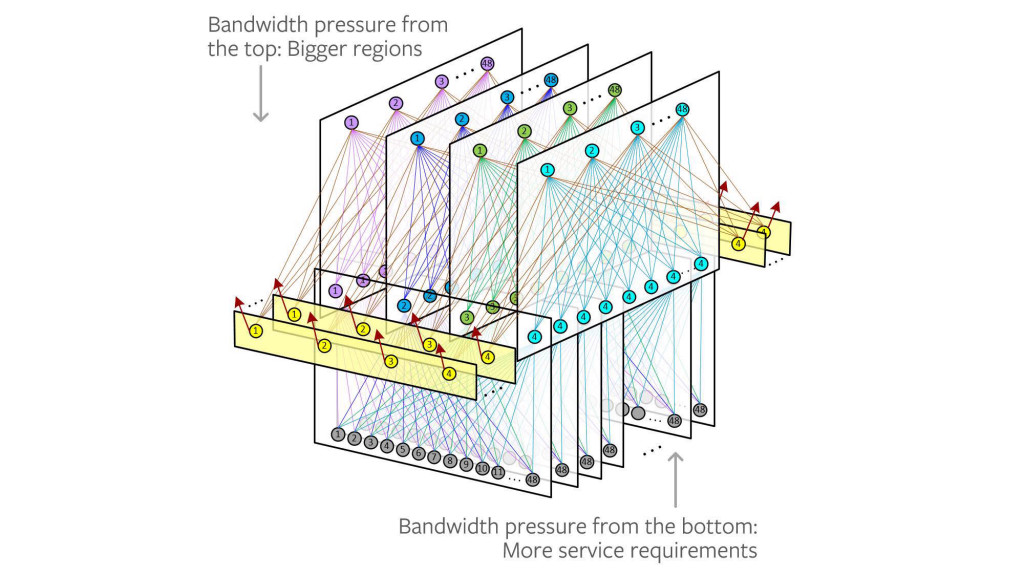
\includegraphics[scale=6]{methodology/images/fb_clos.jpg}
\caption[DC Clos Network]{Data Center Clos Cluster Network Fabric. The four planes at the top aggregate the communication links from each rack. The nodes shown at the top of the plane indicate aggregation switches and the nodes shown at the bottom indicate each rack's TOR switch. The lower planes represent server racks, with the gray nodes indicating individual servers. In this arrangement each rack's TOR switch has four logical links, with each link densely connected to all switches in the isolated aggregation planes. The yellow planes represent the edge of the cluster network, it provides communication with remote clusters and external systems. Image from  \cite{fb_clos}.}
\label{img_fb_clos}
\end{figure}